\documentclass{article}
\usepackage[polish]{babel}
\usepackage[OT4]{fontenc}
\usepackage[utf8]{inputenc}
\usepackage{hyperref}
\usepackage{graphicx}
\usepackage{float}
\usepackage{amsmath}
\usepackage{indentfirst}

\title{\textbf{Praca projektowa z przedmiotu Sztuczna Inteligencja}}
\author{Bartłomiej Czajka 169522 2 EF-DI P1}
\date{Rzeszów, 2023}
\linespread{1.5}
\begin{document}
\maketitle
\pagebreak



\tableofcontents{}
\section{Opis projektu}
\subsection{Założenia projektowe}
Celem projektu jest realizacja sieci neuronowej uczonej za pomocą algorytmu sieci głębokiej, klasyfikującej chorobę Parkinsona oraz zbadanie wpływu parametrów sieci na proces uczenia.
Projekt został zrealizowany w języku Python z wykorzystaniem biblioteki PyTorch.
\subsection{Zestaw danych}
Zestaw danych uczących został pobrany ze strony \href{http://archive.ics.uci.edu/ml/datasets/Parkinsons}{http://archive.ics.uci.edu/ml/datasets/Parkinsons}.
Zawiera on 197 instancji, 23 cechy oraz 2 klasy. Dane są nieuporządkowane, nie ma danych nieokreślonych.
Dokładniejszy opis cech zestawu:
\begin{itemize}
    \item name - Nazwa badanego pacjenta w ASCII i numer nagrania.
    \item MDVP:Fo(Hz) - Średnia częstotliwość podstawowa głosu.
    \item MDVP:Fhi(Hz) - Maksymalna częstotliwość podstawowa głosu.
    \item MDVP:Flo(Hz) - Minimalna częstotliwość podstawowa głosu.
    \item MDVP:Jitter(\%), MDVP:Jitter(Abs), MDVP:RAP, MDVP:PPQ, Jitter:DDP - Kilka miar zmienności częstotliwości podstawowej.
    \item MDVP:Shimmer, MDVP:Shimmer(dB), Shimmer:APQ3, Shimmer:APQ5, MDVP:APQ, Shimmer:DDA - Kilka miar zmienności amplitudy.
    \item NHR, HNR - Dwie miary stosunku szumu do składowych tonalnych w głosie.
    \item status - Stan zdrowia badanego (jeden) - chory na Parkinsona, (zero) - zdrowy.
    \item RPDE, D2 - Dwie miary złożoności dynamicznej nieliniowej.
    \item DFA - Wykładnik skalowania fraktalnego sygnału.
    \item spread1, spread2, PPE - Trzy nieliniowe miary zmienności częstotliwości podstawowej.
\end{itemize}
\subsection{Przygotowanie danych}
Sieć ma za zadanie sklasyfikować czy pacjent cierpi na chorobę Parkinsona. Wartość '1' oznacza osobę cierpiącą na chorobę Parkinsona, natomiast '0' oznacza osobę zdrową.
Dane zostały uporządkowane i znormalizowane.
Normalizacja została wykonana dla każdej obserwacji przy użyciu wzoru:
\[
    x_{\text{norm}} = \frac{{x_{\text{norm\_max}} - x_{\text{norm\_min}}}}{{x_{\text{max}} - x_{\text{min}}}} \cdot (x - x_{\text{min}}) + x_{\text{norm\_min}}
\]

gdzie:
\begin{itemize}
    \item $x_{min}$ - to wektor zawierający minimalne wartości dla każdej obserwacji.
    \item $x_{max}$ - to wektor zawierający maksymalne wartości dla każdej obserwacji.
    \item $x_{norm\_min}$ - to wartość minimalna po normalizacji (-1).
    \item $x_{norm\_max}$ - to wartość maksymalna po normalizacji (1).
    \item $x_{norm}$ - to macierz zawierająca znormalizowane dane.
    \item $x$ - to macierz zawierająca dane wejściowe.
\end{itemize}
\section{Zagadnienia teoretyczne}
\subsection{Matematyczny opis sztucznego neuronu}
Podstawowym elementem budującym strukturę sieci neuronowej jest neuron. Jest to element, który przetwarza informacje.
W pewnym, uproszczonym stopniu jest wzorowany na funkcjonowaniu biologicznej komórki nerwowej.
Struktura neuronu zawiera wiele wejść oraz jedno wyjście.
Jednym z najważniejszych składników neuronu są wagi, których wartości decydują o zachowaniu neuronu. Są one zazwyczaj ustalane w trakcie procesu uczenia.
\begin{figure}[H]
    \centering
    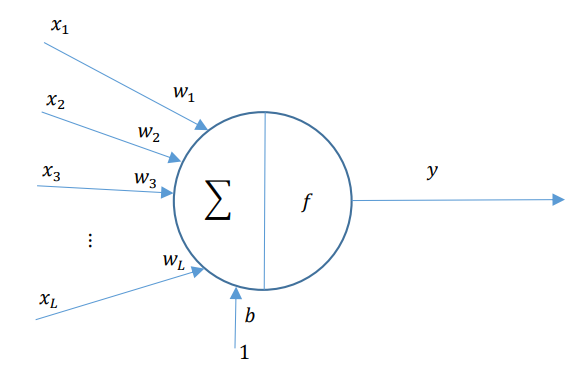
\includegraphics[width=0.8\textwidth, keepaspectratio]{model_neuronu.png}
    \caption{Model neuronu [4]}
    \label{fig:zdjecie}
\end{figure}

Każdy pojedynczy neuron przyjmuje sygnały wejściowe, które są następnie przetwarzane.
Każde wejście ma przypisany współczynnik wagowy, który określa jak bardzo wpływa ono na wynik neuronu.
Ponadto, neuron posiada "bias", czyli dodatkowe wejście, na którym występuje stała wartość.
Wszystkie te informacje są sumowane, aby obliczyć łączne pobudzenie neuronu.
Następnie wartość pobudzenia przechodzi przez funkcję aktywacji, która określa sygnał wyjściowy neuronu.

Wzór na łączne pobudzenie neuronu:
\[
    y = \sum_{j=1}^{L} f(w_{j} x_{j} + b)
\]

gdzie:
\begin{itemize}
    \item $j$ -- indeks, który przyjmuje wartości od 1 do $L$,
    \item $y$ -- wyjście neuronu,
    \item $w_{j}$ -- współczynnik wagowy przypisany do $j$-tego wejścia,
    \item $x_{j}$ -- $j$-ty sygnał wejściowy,
    \item $b$ -- bias [2].
\end{itemize}

\subsection{Funkcja aktywacji}
Sam model matematyczny neuronu nie byłby wystarczający do skomplikowanych obliczeń w m.in. sieciach głębokich.
Należy wprowadzić funkcje aktywacji, które nadają sieciom neuronowym zdolność modelowania nieliniowych relacji między danymi wejściowymi, a wyjściowymi.
Dzięki tej nieliniowej transformacji na wyjściu sztucznego neuronu, możliwe jest wprowadzenie nieliniowości i bardziej skomplikowanych obliczeń.

Istnieje wiele funkcji aktywacji.
Szczególnie przydatną w modelach głębokich ze względu na swoją prostotę i skuteczność jest funkcja ReLU, która została przeze mnie wykorzystana jako funkcja aktywacji dla warstw ukrytych.
Działa na zasadzie przekazywania wartości dodatnich bez ich zmiany, natomiast dla wartości ujemnych przypisuje zerową wartość.
Matematycznie można zdefiniować ją następującym wzorem:
\[
    f(x) = \max(0, x)
\]
Innymi słowy, funkcja ReLU jest zdefiniowana na przedziale:
\[
    f(x) = \begin{cases}
        0, & \text{gdy } x \leq 0, \\
        x, & \text{gdy } x > 0.
    \end{cases}
\]
gdzie:
\begin{itemize}
    \item $x$ -- wartość wejściowa, na której zostanie zastosowana funkcja aktywacji.
\end{itemize}

Istnieje również funkcja aktywacji softmax, która dla danego wektora wyników \( \mathbf{z} = (z_1, z_2, \ldots, z_n) \), gdzie \( n \) oznacza liczbę klas, przekształca każdy element \( z_i \) na wartość prawdopodobieństwa \( p_i \).
Funkcję softmax można zdefiniować w następujący sposób:
\[
    f(z)_i = \frac{e^{z_i}}{\sum_{j=1}^{n} e^{z_j}}
\]
gdzie:
\begin{itemize}
    \item \(f(z)_i\) -- \(i\)-ty element wyniku funkcji softmax dla wektora wyników \(\mathbf{z}\),
    \item \(e^{z_i}\) -- funkcja wykładniczą podniesiona do potęgi \(z_i\),
    \item \(z_i\) -- \(i\)-ty element wektora wyników,
    \item \(\sum_{j=1}^{n} e^{z_j}\) -- suma funkcji wykładniczych dla wszystkich elementów wektora wyników,
    \item \(n\) -- liczba klas.
\end{itemize}
Ostatnią funkcją aktywacji, którą wykorzystałem, jest funkcja sigmoidalna.
Analogicznie do funkcji softmax, została użyta do aktywacji warstwy wyjściowej.
Funkcja sigmoidalna przekształca wartość wejściową na wartość z zakresu (0, 1), co czyni ją przydatną w problemach klasyfikacji binarnej.
Matematycznie funkcję sigmoidalną można zdefiniować jako:
\[
    f(x) = \frac{1}{1 + e^{-x}}
\]
gdzie:
\begin{itemize}
    \item \(x\) -- wartość wejściowa do funkcji sigmoidalnej,
    \item \(e\) --  podstawa logarytmu naturalnego, przybliżone do wartości 2.71828,
    \item \(f(x)\) -- to wartość wyjściowa funkcji sigmoidalnej, przekształcająca \(x\) na wartość z przedziału (0, 1).
\end{itemize}
\subsection{Sieć głęboka}
Sieci głębokie to rodzaj modeli uczenia maszynowego, które składają się z wielu warstw neuronów, zwanych warstwami głębokimi.
Uczenie sieci głębokich opiera się na zasadzie propagacji wstecznej, która jest jednym z kluczowych algorytmów używanych do dostosowania wag sieci neuronowej w procesie uczenia.
Propagacja wsteczna umożliwia obliczenie gradientów wag sieci na podstawie funkcji celu i propaguje te gradienty wstecz przez sieć, aby zaktualizować wagi w celu minimalizacji błędu.
\begin{figure}[H]
    \centering
    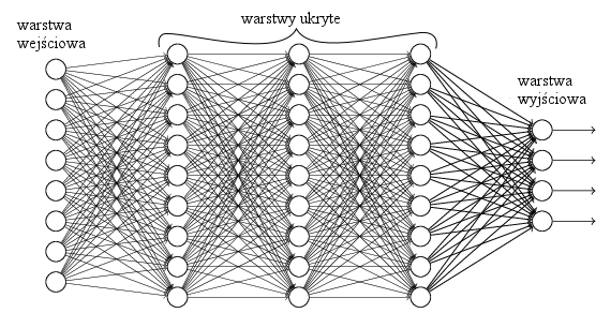
\includegraphics[width=1\textwidth, keepaspectratio]{siec_gleboka.png}
    \caption{Sieć głęboka [5]}
    \label{fig:siec}
\end{figure}


Proces uczenia sieci głębokich rozpoczyna się od inicjalizacji wag, które mogą być inicjalizowane losowo lub przy użyciu innych metod.
Następnie dane wejściowe są przekazywane od warstwy wejściowej do warstwy wyjściowej (ang. forward propagation).
Każda warstwa na podstawie wag i funkcji aktywacji oblicza swoje wyjście.
Na podstawie wyników obliczana jest wartość funkcji kosztu, która mierzy błąd przewidywań sieci.
Kolejnym krokiem jest wykorzystanie algorytmu propagacji wstecznej, który oblicza gradienty wag sieci neuronowej.
Gradienty oblicza się iteracyjnie, zaczynając od warstwy wyjściowej przechodząc wstecz przez kolejne warstwy sieci.
W dalszej kolejności, biorąc pod uwagę obliczone gradienty wag, wagi sieci są aktualizowane w celu zminimalizowania funkcji kosztu mierzącej błąd predykcji sieci.
Dokonuje się tego za pomocą optymalizatora (np. ADAM).
Wyżej wymienione kroki powtarza się aż do osiągnięcia zdefiniowanej liczby epok lub innych kryteriów zatrzymania.
\subsection{Funkcja kosztu}
Wykorzystaną funkcją kosztu w programie jest entropia krzyżowa.
Funkcja ta mierzy stopień niezgodności między rzeczywistymi etykietami, a przewidywanymi prawdopodobieństwami dla każdej klasy.
Im większa niezgodność, tym większa wartość funkcji kosztu.
Dąży się do minimalizacji tej funkcji, poprzez zmianę wag sieci.

Entropię krzyżową, w szczególności dla klasyfikacji binarnej, można zdefiniować następującym wzorem:
\[
    H(y, p) = -\sum_{i=1}^{C} y_i \log(p_i) = -\sum_{i=1}^{2} y_i \log(p_i) = -[y_1 \log(p_1) + y_2 \log(p_2)] = - [y \log(p) + (1-y) \log(1-p)]
\]
gdzie:
\begin{itemize}
    \item  \(H(y, p)\) -- wartość entropii krzyżowej,
    \item  \(y_i\) -- \(i\)-ta rzeczywista etykieta (0 lub 1) dla próbki i,
    \item  \(p_i\) -- \(i\)-te przewidziane prawdopodobieństwo dla próbki i,
    \item \(C\) -- liczba klas.
\end{itemize}

Aby obliczyć gradient funkcji kosztu, można użyć propagacji wstecznej błędu.

\[\frac{\partial H}{\partial z_i} = p_i - y_i\]

\begin{itemize}
    \item \(\frac{\partial H}{\partial z_i}\) to gradient funkcji kosztu względem wejścia \(z_i\) do funkcji aktywacji (np. softmax) w warstwie wyjściowej,
    \item \(p_i\) to przewidywane prawdopodobieństwo dla próbki \(i\),
    \item \(y_i\) to rzeczywista etykieta (0 lub 1) dla próbki \(i\).
\end{itemize}
Następnie ten gradient jest propagowany wstecz przez warstwy ukryte, aż do warstwy wejściowej, gdzie obliczane są gradienty względem wag sieci.
W praktyce, algorytm propagacji wstecznej błędu jest stosowany do obliczenia gradientów dla wszystkich parametrów sieci, a następnie te gradienty są wykorzystywane w procesie optymalizacji, na przykład przy użyciu algorytmu ADAM, aby dostosować wagi sieci i minimalizować funkcję kosztu.


\subsection{Algorytm wstecznej propagacji błędu}
Algorytm wstecznej propagacji błędu, nazywany również algorytmem największego spadku gradientu, jest jednym z głównych algorytmów stosowanych w procesie uczenia sieci głębokich.
Umożliwia on aktualizację wag sieci w celu minimalizacji funkcji kosztu poprzez iterację przez kolejne warstwy sieci.
Proces ten można podzielić na dwa kroki: propagację w przód oraz wstecz.

Propagacja w przód polega na przekazywaniu danych wejściowych przez sieć od warstwy wejściowej do warstwy wyjściowej.
W każdej warstwie obliczane są aktywacje neuronów na podstawie obecnych wag i danych wejściowych.
Wyniki z danej warstwy przekazywane są do kolejnej aż do warstwy wyjściowej gdzie generowany jest wynik predykcji.

W propagacji wstecznej natomiast porównuje się wynik sieci z oczekiwanym wynikiem, obliczając przy tym błąd.
Błąd ten jest następnie propagowany wstecz od zaczynając od warstwy wyjściowej.
Obliczany jest gradient funkcji kosztu względem wag sieci, który informuje o kierunku dostosowania wag w celu minimalizacji błędu.
Na podstawie gradientu aktualizowane są wagi sieci przy użyciu odpowiedniej metody optymalizacji, takiej jak metoda spadku gradientu czy też jej wariant, np. ADAM.
\subsection{Metoda optymalizacji ADAM}
Metoda ADAM jest popularna w optymalizacji sieci głębokich, ponieważ łączy zalety adaptacyjnego skalowania kroku uczenia (RMSProp) i momentu, co prowadzi do efektywniejszej optymalizacji i szybszego zbiegania do optymalnych wag sieci.

Wzór na gradient funkcji kosztu w metodzie ADAM można zapisać następująco:

\[g_t = \nabla_{\theta} J(\theta)\]
gdzie:
\begin{itemize}
    \item \(g_t\) to gradient w kroku czasowym \(t\),
    \item \(\nabla_{\theta}\) oznacza gradient po wagach \(\theta\),
    \item \(J(\theta)\) to funkcja kosztu.
\end{itemize}
Gradient jest obliczany za pomocą standardowych metod propagacji wstecznej błędu w sieciach neuronowych.
\begin{enumerate}
    \item Obliczenie gradientów funkcji kosztu względem wag sieci za pomocą propagacji wstecznej błędu.
    \item Aktualizacja momentu gradientu \(m_t\) i drugiego momentu gradientu \(v_t\) na podstawie obliczonych gradientów.
    \item Obliczenie wygładzonych estymacji momentu i drugiego momentu: \(\hat{m}_t\) i \(\hat{v}_t\).
    \item Aktualizacja wag sieci z wykorzystaniem estymacji momentu i drugiego momentu, współczynnika uczenia \(\alpha\) oraz małej wartości epsilon \(\epsilon\).
\end{enumerate}

W metodzie ADAM, gradient jest używany do aktualizacji wag zgodnie z następującymi wzorami:
\[m_t = \beta_1 \cdot m_{t-1} + (1 - \beta_1) \cdot g_t\]
\[v_t = \beta_2 \cdot v_{t-1} + (1 - \beta_2) \cdot g_t^2\]
\[\hat{m}_t = \frac{m_t}{1 - \beta_1^t}\]
\[\hat{v}_t = \frac{v_t}{1 - \beta_2^t}\]
\[\theta_{t+1} = \theta_t - \alpha \cdot \frac{\hat{m}_t}{\sqrt{\hat{v}_t} + \epsilon}\]

gdzie:
\begin{itemize}
    \item \(m_t\) to estymacja momentu gradientu w kroku czasowym \(t\).
    \item \(v_t\) to estymacja drugiego momentu gradientu w kroku czasowym \(t\).
    \item \(\beta_1\) i \(\beta_2\) to współczynniki z zakresu \([0, 1)\) kontrolujące eksponencjalne wygładzanie momentu i drugiego momentu.
    \item \(\alpha\) to współczynnik uczenia (learning rate).
    \item \(\epsilon\) to mała wartość (np. \(10^{-8}\)) używana w celu uniknięcia dzielenia przez zero.
    \item \(\hat{m}_t\) i \(\hat{v}_t\) to wygładzone estymacje momentu i drugiego momentu.
    \item \(\theta_t\) i \(\theta_{t+1}\) to wagi w krokach czasowych \(t\) i \(t+1\) odpowiednio.
\end{itemize}
Przy użyciu tych równań, algorytm ADAM aktualizuje wagi sieci neuronowej, wykorzystując estymację momentu i drugiego momentu gradientu.
To pozwala na efektywną optymalizację sieci głębokiej, dostosowując krok uczenia (learning rate) dla każdej wagi indywidualnie.
\section{Realizacja sieci neuronowej}
\subsection{Opis skryptu}
\section{Eksperymenty}
\subsection{Eksperyment 1}
\subsection{Eksperyment 2}
\subsection{Eksperyment 3}
\section{Wnioski}
\begin{thebibliography}{9}
    \bibitem{Nielsen}
    Michael Nielsen,
    \emph{Neural Networks and Deep Learning}.
    Determination Press,
    2015.
    \bibitem{TadeusiewiczSzaleniec}
    Ryszard Tadeusiewicz, Maciej Szaleniec,
    \emph{Leksykon sieci neuronowych}.
    Wrocław,
    2015.
    \bibitem{vandeput}
    Nicolas Vandeput,
    \href{https://medium.com/analytics-vidhya/a-brief-history-of-neural-networks-c234639a43f1}{\emph{A Brief History Of Neural Networks}},
    [dostęp: 17.05.2023].
    \bibitem{zajdel}
    Zajdel R.,
    \emph{Ćwiczenie 4 Model Neuronu},
    Rzeszów,
    KIiA, PRz.
    \bibitem{gora}
    Paweł Gora,
    \href{https://www.deltami.edu.pl/temat/informatyka/sztuczna_inteligencja/2017/12/28/Glebokie_uczenie_maszyn/}{\emph{Głębokie uczenie maszyn}},
    [dostęp: 17.05.2023].
    \bibitem{zajdel}
    Zajdel R.,
    \emph{Procedura przygotowania danych dla sieci neuronowych na potrzeby projektu z modułu sztuczna inteligencja - Listing1},
    Rzeszów,
    KIiA, PRz.
    \bibitem{zajdel}
    Zajdel R.,
    \emph{Procedura przygotowania danych dla sieci neuronowych na potrzeby projektu z modułu sztuczna inteligencja - Listing2},
    Rzeszów,
    KIiA, PRz.
\end{thebibliography}
\end{document}